\subsection{Memory model}

OpenMP supports a \textbf{shared memory model}. It is a model where \textbf{all threads share an address space}, but it can get complicated, for example in the following example (picture) we can see a shared space that is also in the cache of process 3; so how can we manage this situation? What are the methods to adapt? Furthermore, what happens when a thread modifies a shared address space? How does the system behave?

\begin{figure}[!htp]
    \centering
    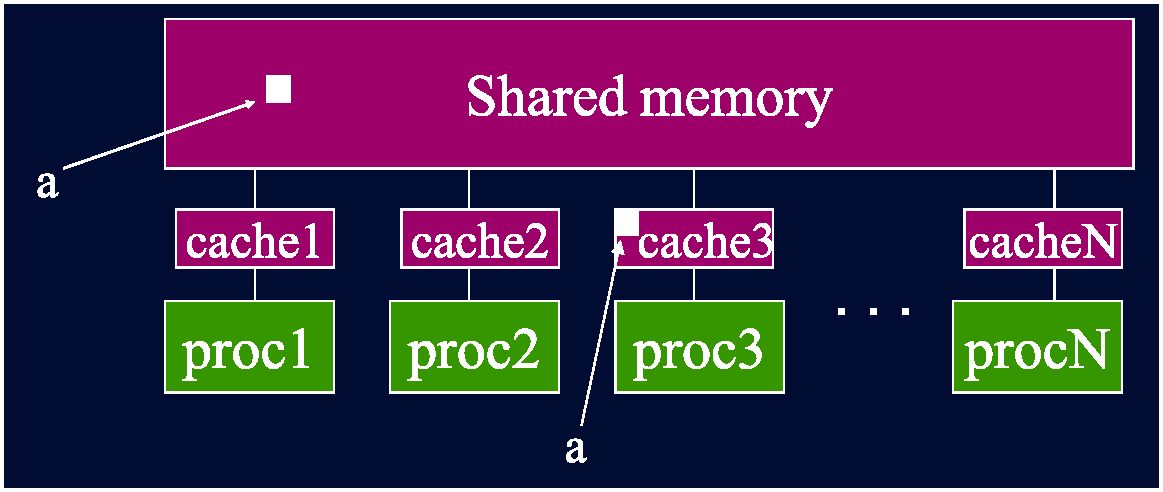
\includegraphics[width=.8\textwidth]{img/memory-model-1.pdf}
\end{figure}

\noindent
In general, a memory model is defined in terms of:
\begin{itemize}
    \item \textbf{\underline{Coherence}}: behavior of the memory system when a \textbf{single address is accessed by multiple threads}.
    \item \textbf{\underline{Consistency}}: read, write, or synchronization (RWS) orders with \textbf{different addresses and through multiple threads}.
\end{itemize}

\begin{remarkbox}[: what the compiler does at the low level]
    When we write a program and ask the compiler to compile it, it does a lot of \dquotes{magic} under the hood.
    \begin{enumerate}
        \item Our source code is decoded into very low level operations. These operations respect the order of the high-level operations of our code.
        \item The compiler, smarter then us, tries to optimize the code while creating the executable code; so it reorders the low-level operations that are \textbf{semantically equivalent} to our program, but often allow to gain performance.
        \item During the execution of the code, if it is parallel, some threads are created and each of them has a private memory address.
        \item Finally, each thread writes/reads from memory, also called the commit order, using some rules.
    \end{enumerate}
    \begin{center}
        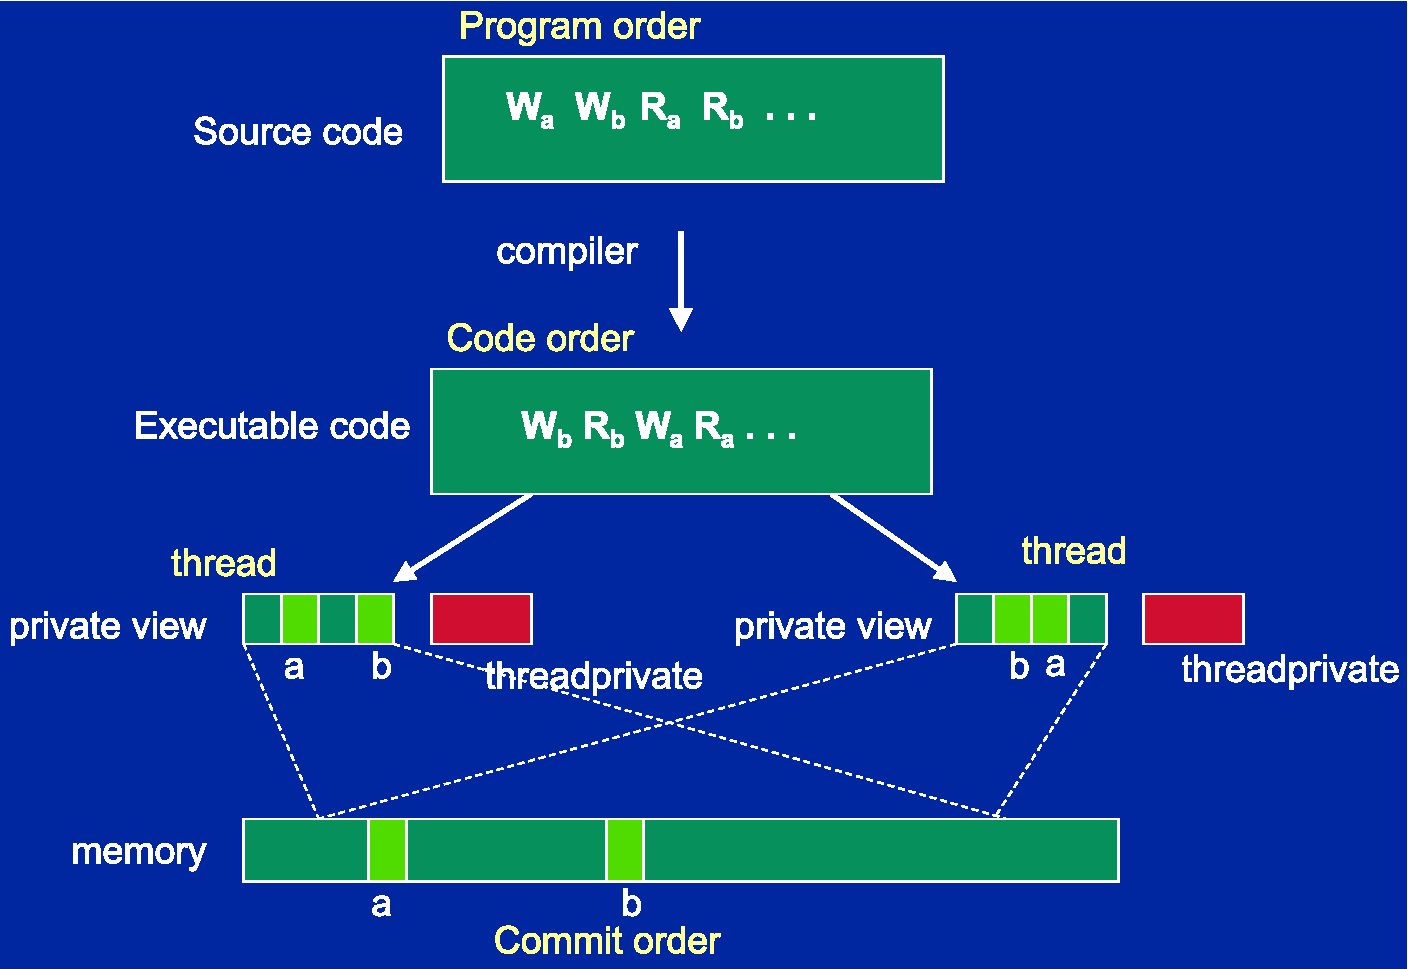
\includegraphics[width=\textwidth]{img/memory-model-2.pdf}
    \end{center}

    Note that the re-ordering are made by:
    \begin{itemize}
        \item \textbf{Compile} re-orders \emph{program order} $\rightarrow$ \emph{code order}.
        \item \textbf{Machine} re-orders \emph{code order} $\rightarrow$ \emph{memory commit order}.
    \end{itemize}
\end{remarkbox}

\noindent
At any given time, the private view seen by a thread may differ from the view in shared memory. For this reason, there are \textbf{consistency models} that \textbf{define constraints on the order of RWS} (Reads, Writes, Synchronizations) \textbf{operations}.

\highspace
In general, a multiprocessor adopts the \textbf{Sequential Consistency Model}. It says that given $n$ operations (RWS), they are sequentially consistent if:
\begin{itemize}
    \item They \textbf{remain in \emph{program order} for each processor}.
    \item They are \textbf{seen to be in the same overall order by each of the other processors}.
\end{itemize}
Also, in a sequential consistency model, program order is the same as code order and commit order.

\highspace
OpenMP uses a \textbf{Relaxed Consistency Model} where the \textbf{compiler cannot reorder synchronization operations with read or write operations on the same thread}. The consequences are:
\begin{itemize}
    \item[\textcolor{Green3}{\ding{51}}] All threads have the same view of memory at specific points in the code, called \textbf{\emph{Consistency Points}}.
    \item[\textcolor{Green3}{\ding{51}}] Between two consistency points, each thread has its own temporary view of memory, which may be different from the other temporary views of other threads.
    \item[\textcolor{Green3}{\ding{51}}] Data are read-only, this guarantee to avoid consistency issues.
    \item[\textcolor{Red2}{\ding{55}}] Shared data that need to be modified can create possible race conditions.
\end{itemize}

\highspace
\textbf{\underline{\texttt{flush} directive}}. Defines a \emph{sequence point} at which a \textbf{thread is guaranteed to see a consistent view of memory} with respect to the \texttt{flush-set}. The \texttt{flush-set} means \emph{\textbf{all thread visible variables}} for a \texttt{flush} construct without an argument list, and it also means a list of variables when the \texttt{flush(list)} construct is used. The action of \texttt{flush} is to \textbf{guarantee} that:
\begin{itemize}
	\item All read/write \textbf{operations that overlap} the \texttt{flush-set} and \textbf{occur \emph{before}} the \texttt{flush} will be \textbf{completed before the \texttt{flush} is executed}.
	
	\item Any read/write \textbf{operations that overlap} the \texttt{flush-set} and \textbf{occur \emph{after}} the \texttt{flush} will \textbf{not be performed until after the \texttt{flush}}.
	
	\item Flushes with overlapping \texttt{flush-set}s can not be reordered.
\end{itemize}
In other words, the \texttt{flush} \textbf{forces data to be updated in memory so that other threads see the most recent value}.
\marginpar{
    \href{https://www.openmp.org/spec-html/5.0/openmpsu96.html\#x127-4920002.17.8} {Doc. \faIcon{book}}
}
\begin{openmpbox}[: \texttt{flush}]
	\begin{lstlisting}[language=C++, mathescape=true]
#pragma omp flush $\emph{flush-set}$\end{lstlisting}
\end{openmpbox}

\noindent
A flush operation is \textbf{implied} by default by OpenMP synchronizations:
\begin{itemize}
	\item At entry/exit of \texttt{parallel}/\texttt{critical} regions;
	\item At implicit and explicit \texttt{barrier}s;
	\item At exit from work-sharing constructs, unless \texttt{nowait} is specified.
\end{itemize}
And it is \textbf{not implied}:
\begin{itemize}
	\item At entry of work-sharing constructs;
	\item At entry and exit of \texttt{master}.
\end{itemize}